\chapter{Experimental Simulation}  

The proposed \gls{bfast} algorithm will be studied using an experimental framework mimicking a single-subject \gls{fmri} experiment. The datasets from this kind of experiment consist of the measured \gls{bold} signal for each voxel throughout the experiment. Also, it contains a structured log of the events during the experiment, which includes, among other things, stimulus times and duration. 

\section{Generation of the Simulated Framework}

\subsection{Selection of True Maps}

The first step to creating a simulated framework is to identify true maps of the activated regions that will be distorted for the simulation. The \gls{bfast} algorithm will then be used to reconstruct the activation maps, and the results will be compared to the original true maps to measure the algorithm's accuracy. In this true maps, each voxel will be assigned a value of 0 if it is not activated and 1 if it is activated. To address different spatial structures, \gls{2d} and \gls{3d} true maps are considered. See Table \ref{tab:aMaps} for more details on the true maps.

\begin{table}[htbp!]
\centering
\caption{Details of True Maps Considered}
\begin{tabular}{x{2.1cm}x{6cm}x{6cm}}
\hline
\textbf{Name} & \textbf{\gls{2d}} & \textbf{\gls{3d}} \\ \hline
Dimensions & $200 \times 200$ & $40 \times 40 \times 25$ \\
Voxels & 40000 & 40000 \\ 
\acrshort{poa} & 19.9375 & 3.9525 \\
Map & 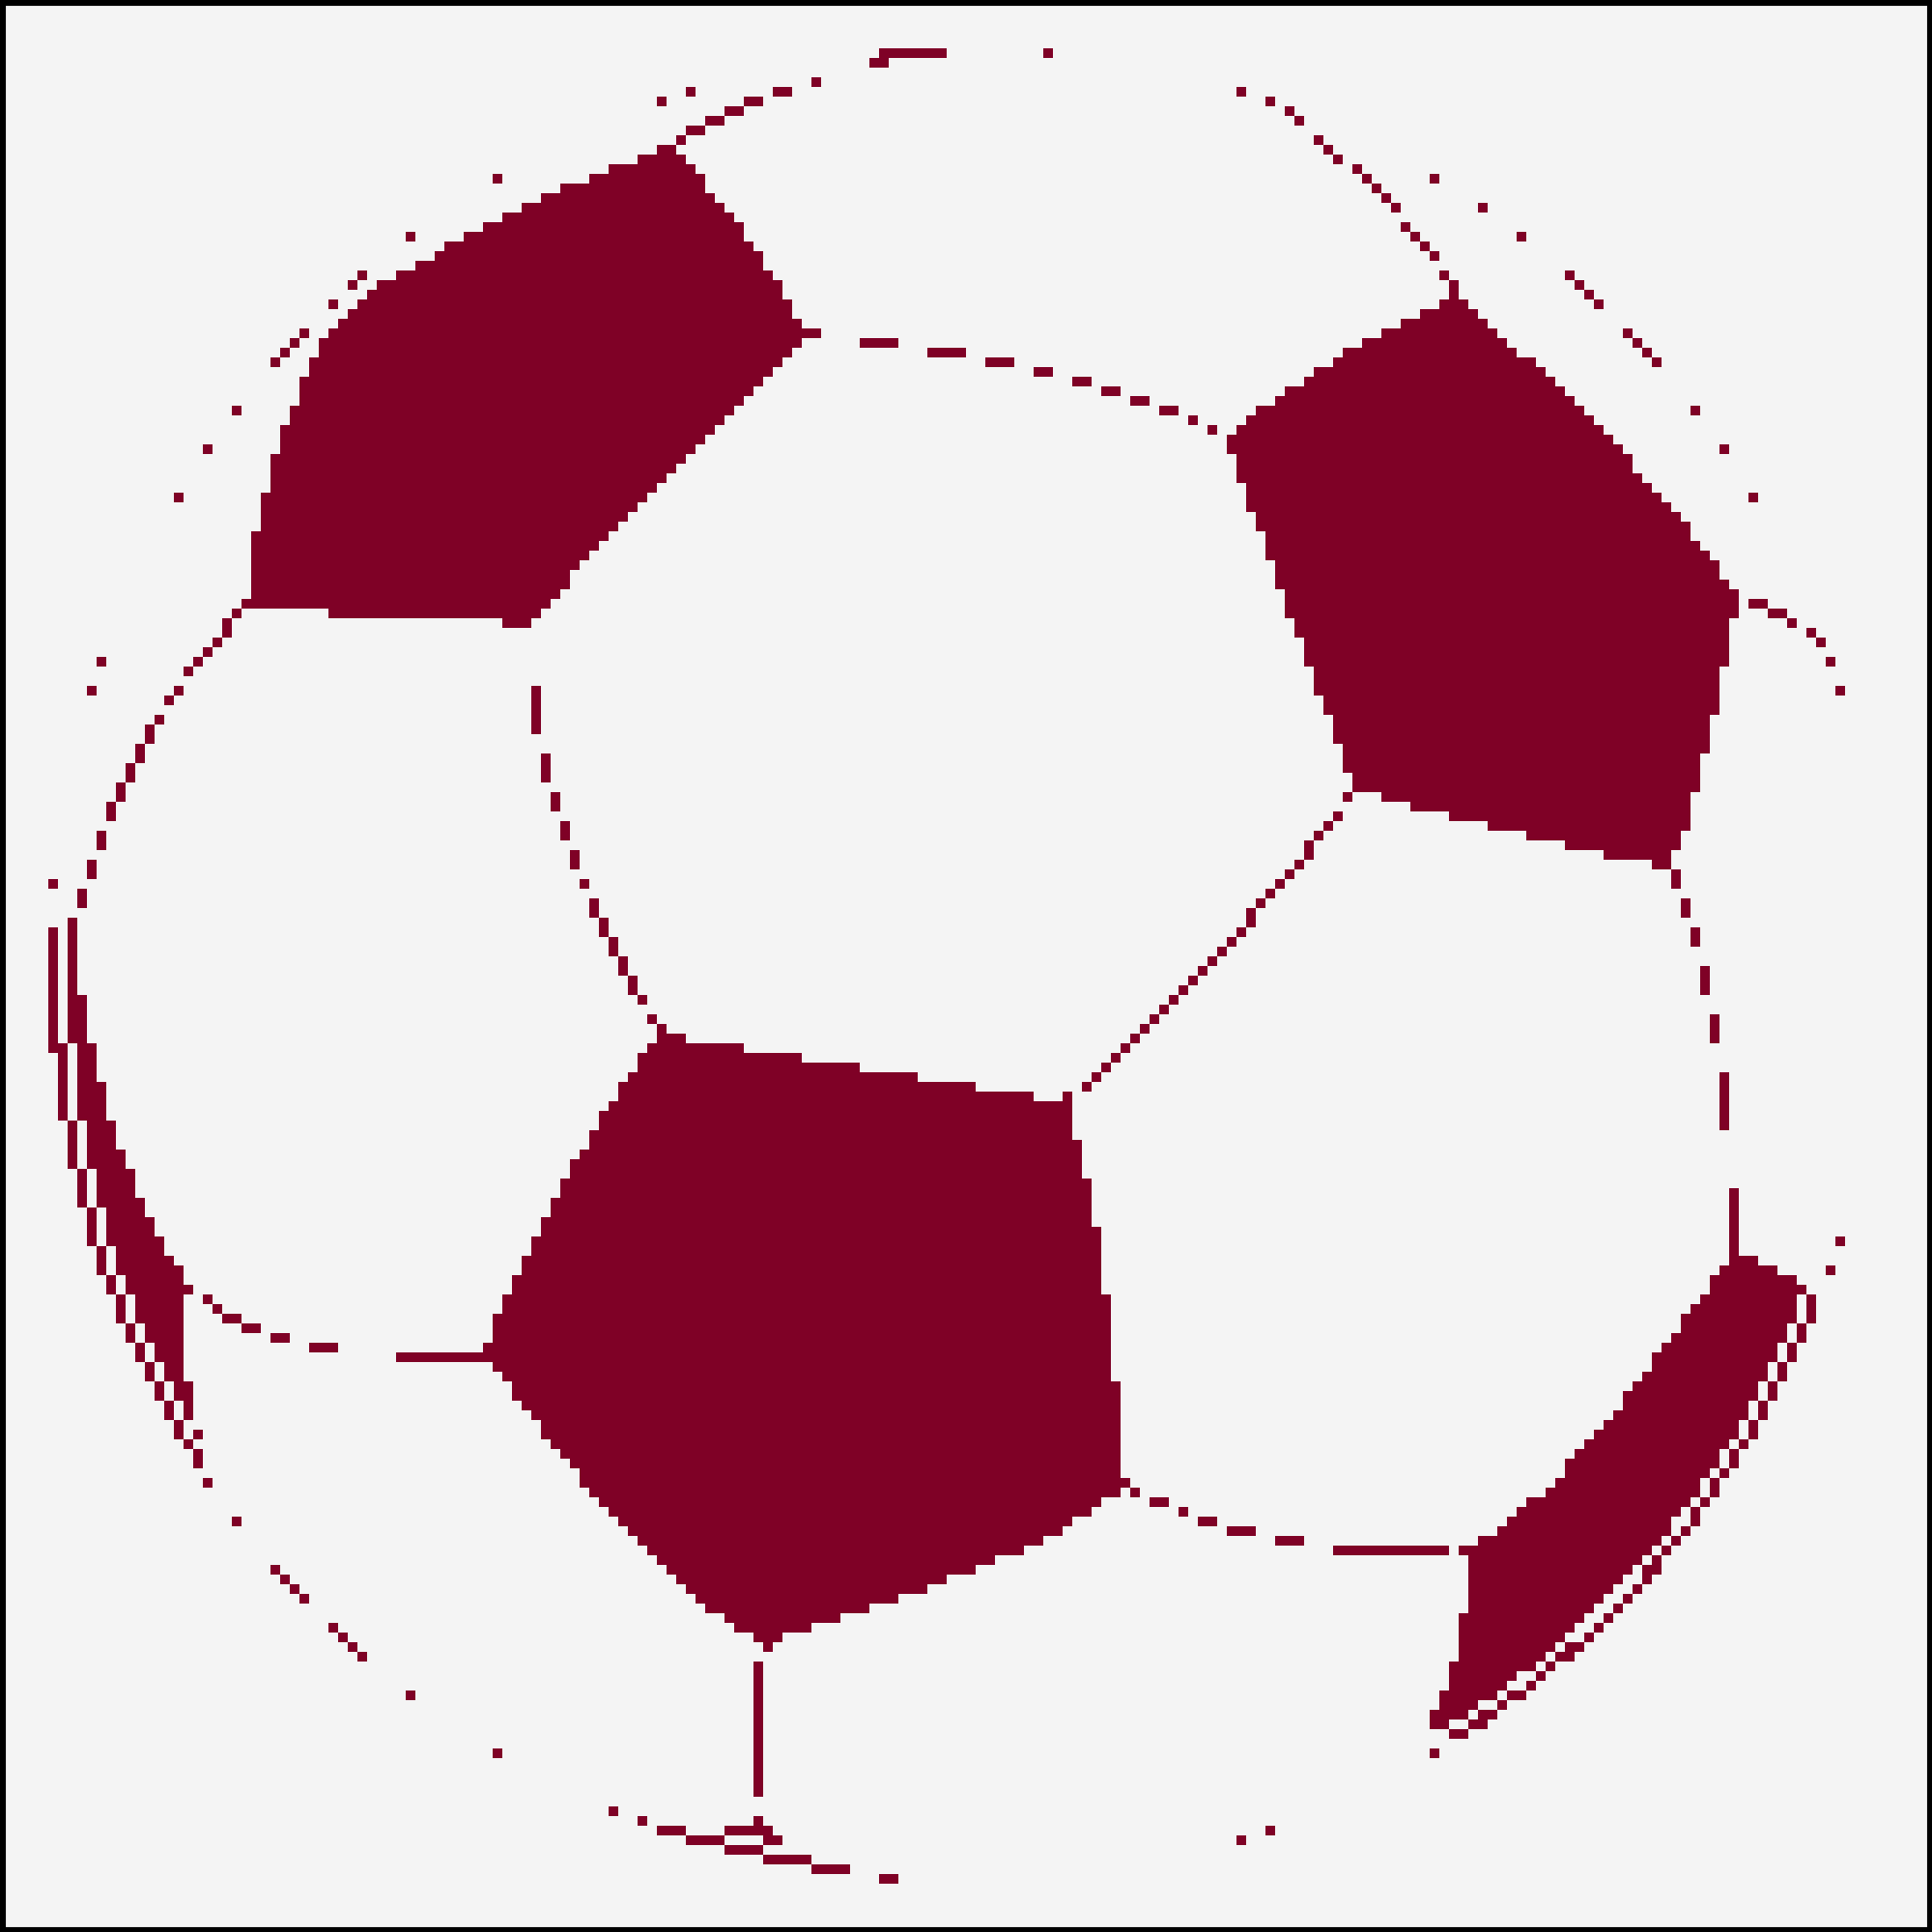
\includegraphics[width=0.35\textwidth]{images/aMap2D.png} & 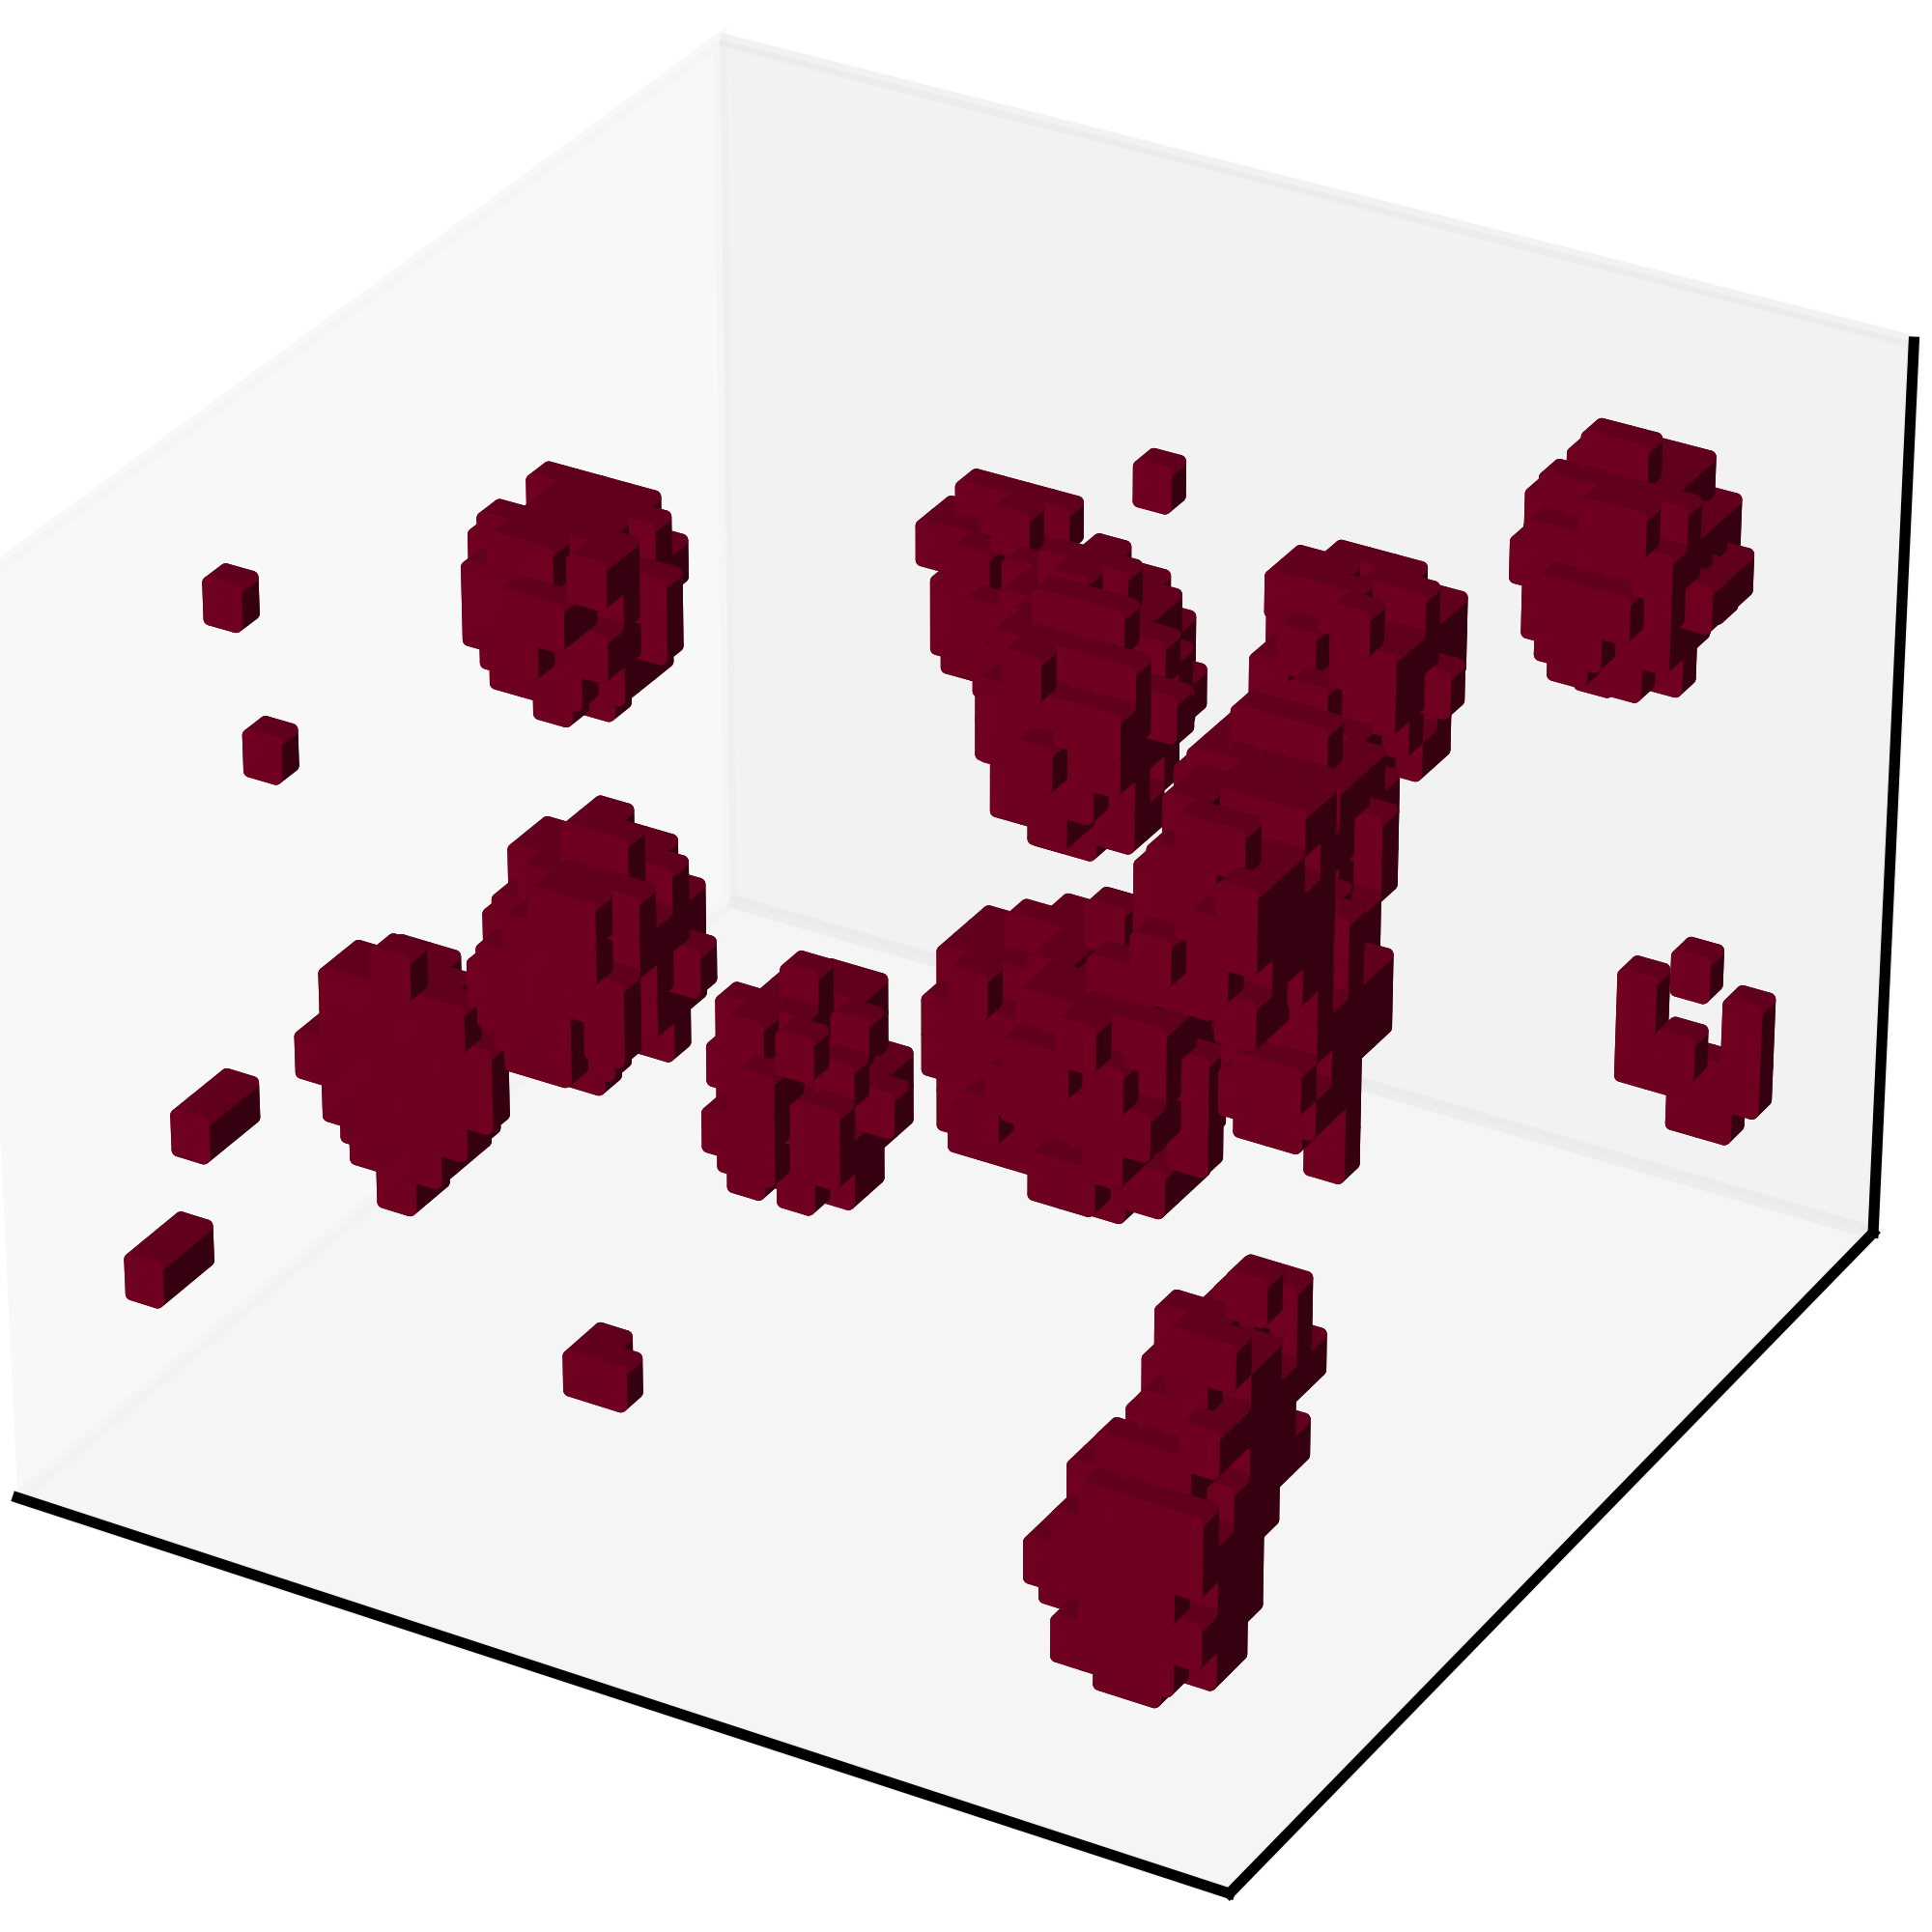
\includegraphics[width=0.35\textwidth]{images/aMap3D.png} \\ 
Source & Derived from File in Open Clip Art Library (Public Domain) & See Appendix \ref{ap:3dMapsGen} \\ \hline
Description & \multicolumn{2}{x{12cm}}{In both maps, dark voxels are active and light voxels are inactive.} \\ \hline
\end{tabular}
\label{tab:aMaps}
\end{table}

\subsection{Creation of Design Matrix}

The next step of the framework-building process is the creation of a design matrix of two columns, $\bm{X}$. The second column corresponds to the constant regressor and the first column contains the Glover \gls{hrf} \cite{lu2006using}, given specific event descriptions of an \gls{fmri} experiment. For the simulated framework, a single type of stimulus will be considered as the event of the \gls{fmri} experiment, however, this event will occur at different times. The scan times and durations were arbitrarily selected as follows:

\begin{table}[htbp!]
\centering
\caption{Event Description of Simulated \gls{fmri} Experiment.}
\begin{tabular}{cc}
\hline
\textbf{Parameter} & \textbf{Value} \\ \hline
Number of Scans & 100 \\
Time Between Scans & 2 seconds \\
Number of Stimulus & 4 \\
Duration of Each Stimulus & 10 seconds \\
Time Between Stimulus & 18 - 25 seconds \\ \hline
\end{tabular}
\label{tab:eventsSim}
\end{table}

Resulting then in the \gls{hrf} shown in Figure \ref{fig:gloverHRF}.

\begin{figure}[htbp!]
\centering
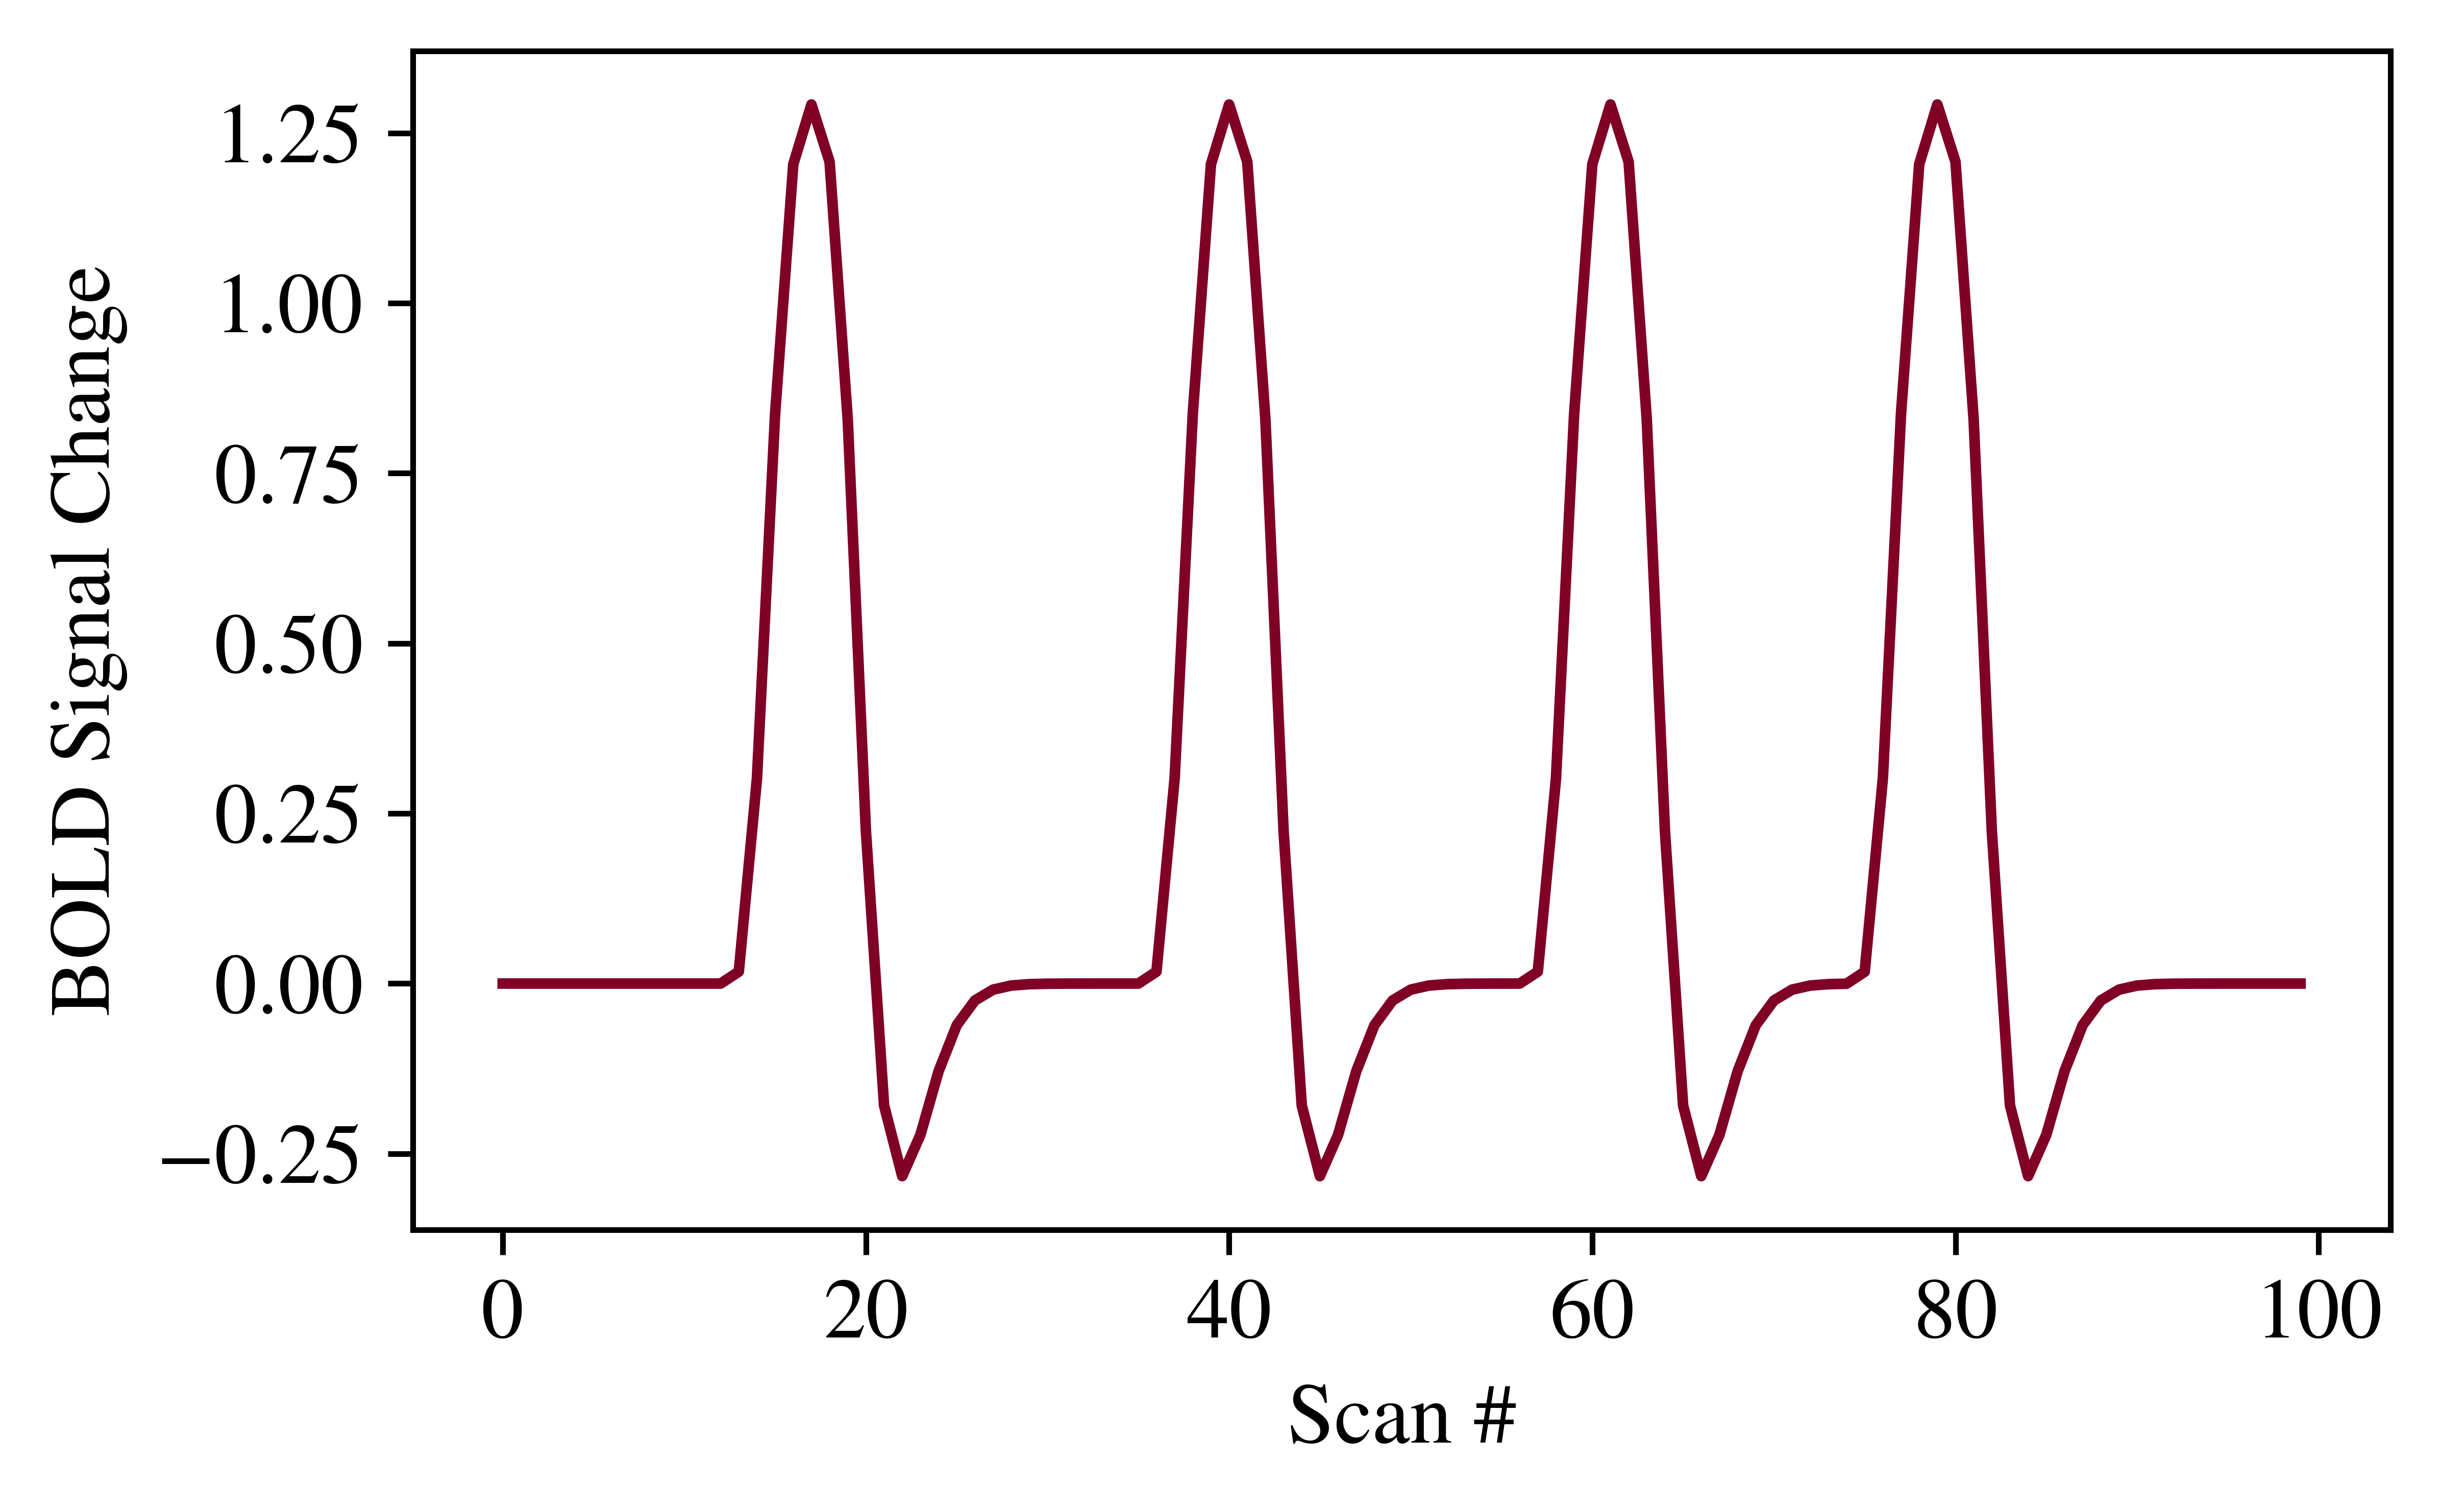
\includegraphics{images/gloverHRF.png}
\caption{Glover \gls{hrf} Given a Stimulus Described by Table \ref{tab:eventsSim}.}
\label{fig:gloverHRF}
\end{figure}

\subsection{Computation of \gls{bold}}

The final step in building the simulated framework is to compute the \gls{bold} response, $\bm{y}_i$, for each voxel $i$. This process is divided into two steps: first, the computation of the \gls{bold} response without noise, and then, using an $ARMA$ Model to generate noise in the signal \cite{choi2012arma}, i.e.:

\begin{equation}
\bm{y}_i = \bm{\hat{y}}_i + \bm{\epsilon}_{\bm{\hat{y}_i}}
\end{equation}

To compute the \gls{bold} response without noise ($\bm{\hat{y}}_i$) we will set values for the parameter $\bm{\beta}_i$ depending on the voxel activation status, $\zeta_i$, on the true map as shown in Table \ref{tab:betaParameter}. The response is then computed as seen in Equation \ref{eq:boldCleanCalc}.

\begin{table}[htbp!]
\centering
\caption{Parameter Selection Based on Activation Status}
\begin{tabular}{cc}
\hline
\textbf{Activation Status} & \textbf{Parameter Values} \\ \hline
$\zeta_i=0$ & $\bm{\beta}_i = (0,100)^T$ \\
$\zeta_i=1$ & $\bm{\beta}_i = (75,100)^T$ \\ \hline
\end{tabular}
\label{tab:betaParameter}
\end{table}

\begin{equation} \label{eq:boldCleanCalc}
\bm{\hat{y}}_i = \bm{X}\bm{\beta}_i
\end{equation}

On the other side, the noise ($\bm{\epsilon}_{\bm{\hat{y}_i}}$) is a vector of mean $\mu_{ARMA} = 0$ and variance $\sigma_{ARMA}^2$ with a baseline structure equivalent to $ARMA_{\bm{\epsilon}_{\bm{\hat{y}_i}}}\left( \{p_1,p_2,\dots\},\{q_1,q_2,\dots\} \right)$. Note that $P = \left| \{p_1,p_2,\dots\} \right|$ and $Q= \left| \{q_1,q_2,\dots\} \right|$ are related to the order of the corresponding $ARMA$ model. Also, $p_a$ and $q_b$ represent the coefficients of such models. Values of $P$ and $Q$ in the range $[0,3]$ were chosen to study the model under different noise scenarios. The values of $\sigma_{ARMA}$, $p_a$, and $q_b$ were chosen arbitrarily as parameters, see Table \ref{tab:noiseParameters}.

\begin{table}[htbp!]
\centering
\caption{Parameter Selection Related to $\bm{\epsilon}_{\bm{\hat{y}_i}}$}
\begin{tabular}{cc}
\hline
\textbf{Order} & \textbf{Values} \\ \hline
All & $\sigma_{ARMA}=25$ \\ 
$P=0$ & Model without Auto-Regression \\ 
$P=1$ & $\{p_1\} = \{0.5\}$ \\ 
$P=2$ & $\{p_1,p_2\} = \{0.5,0.3\}$ \\ 
$P=3$ & $\{p_1,p_2,p_3\} = \{0.5,0.3,0.1\}$ \\
$Q=0$ & Model without Moving-Average \\ 
$Q=1$ & $\{q_1\} = \{0.5\}$ \\ 
$Q=2$ & $\{q_1,q_2\} = \{0.5,0.3\}$ \\ 
$Q=3$ & $\{q_1,q_2,q_3\} = \{0.5,0.3,0.1\}$ \\\hline
\end{tabular}
\label{tab:noiseParameters}
\end{table}